\subsection{Support Vector Machine} \label{svm}

Support Vector Machines (SVM) are highly used due to high empirical performance and somewhat-simple computational complexity, being binary classifiers that when allied with strategies, such as \textit{one-vs-all}, can be expanded to become multi-class classifiers.

In our case, SVM was our first approach to the face detection problem, because the dataset, even after the process of data augmentation, is not very large and we are dealing with a binary classification problem, so we decided to start our initial approach with a simpler model like SVM.

Initially we divide our data in two subsets: training subset with \(80\%\) of the images and testing subset with \(20\%\) of the images.

In SVM there are two main hyper-parameters that can be tweaked to improve the performance of the model, C and Gamma. To get the best performance out of the model we made every combination possible for C and gamma, starting with one of the values present in table \ref{table:svm-initial-configuration}.

\begin{table}[htbp]
\centering
\caption{SVM - Initial Configuration}
\begin{tabular}{ |c|c| } 
 \hline
 \textbf{Train Data} & 80\% \\ 
 \hline
 \textbf{Test Data} & 20\% \\ 
 \hline
 \textbf{Gamma} & [100, 33, 10, 3, 1, 0.3, 0.1, 0.03 ] \\ 
 \hline
 \textbf{C} & [0.01, 0.03, 0.1, 0.3, 1, 3, 10, 30] \\ 
 \hline
\end{tabular}
\label{table:svm-initial-configuration}
\end{table}

To validate which combination of hyper-parameters enabled the best performance out of our model we used K-Fold Cross Validation where our training set was divided in \(K = 5\) smaller sets, where 4 were used for training and 1 was used to validate the model. With this approach we didn't need to reduce the training dataset by creating a validation dataset and the results did not depend on a particular random choice for the pair of (train, validation) datasets.

After validating every combination, as we can see in figure \ref{fig:svm-cross-validation}, the values of C and gamma where our model performed the best are: C = 30 and Gamma = 1.

\begin{figure}[htbp]
\centerline{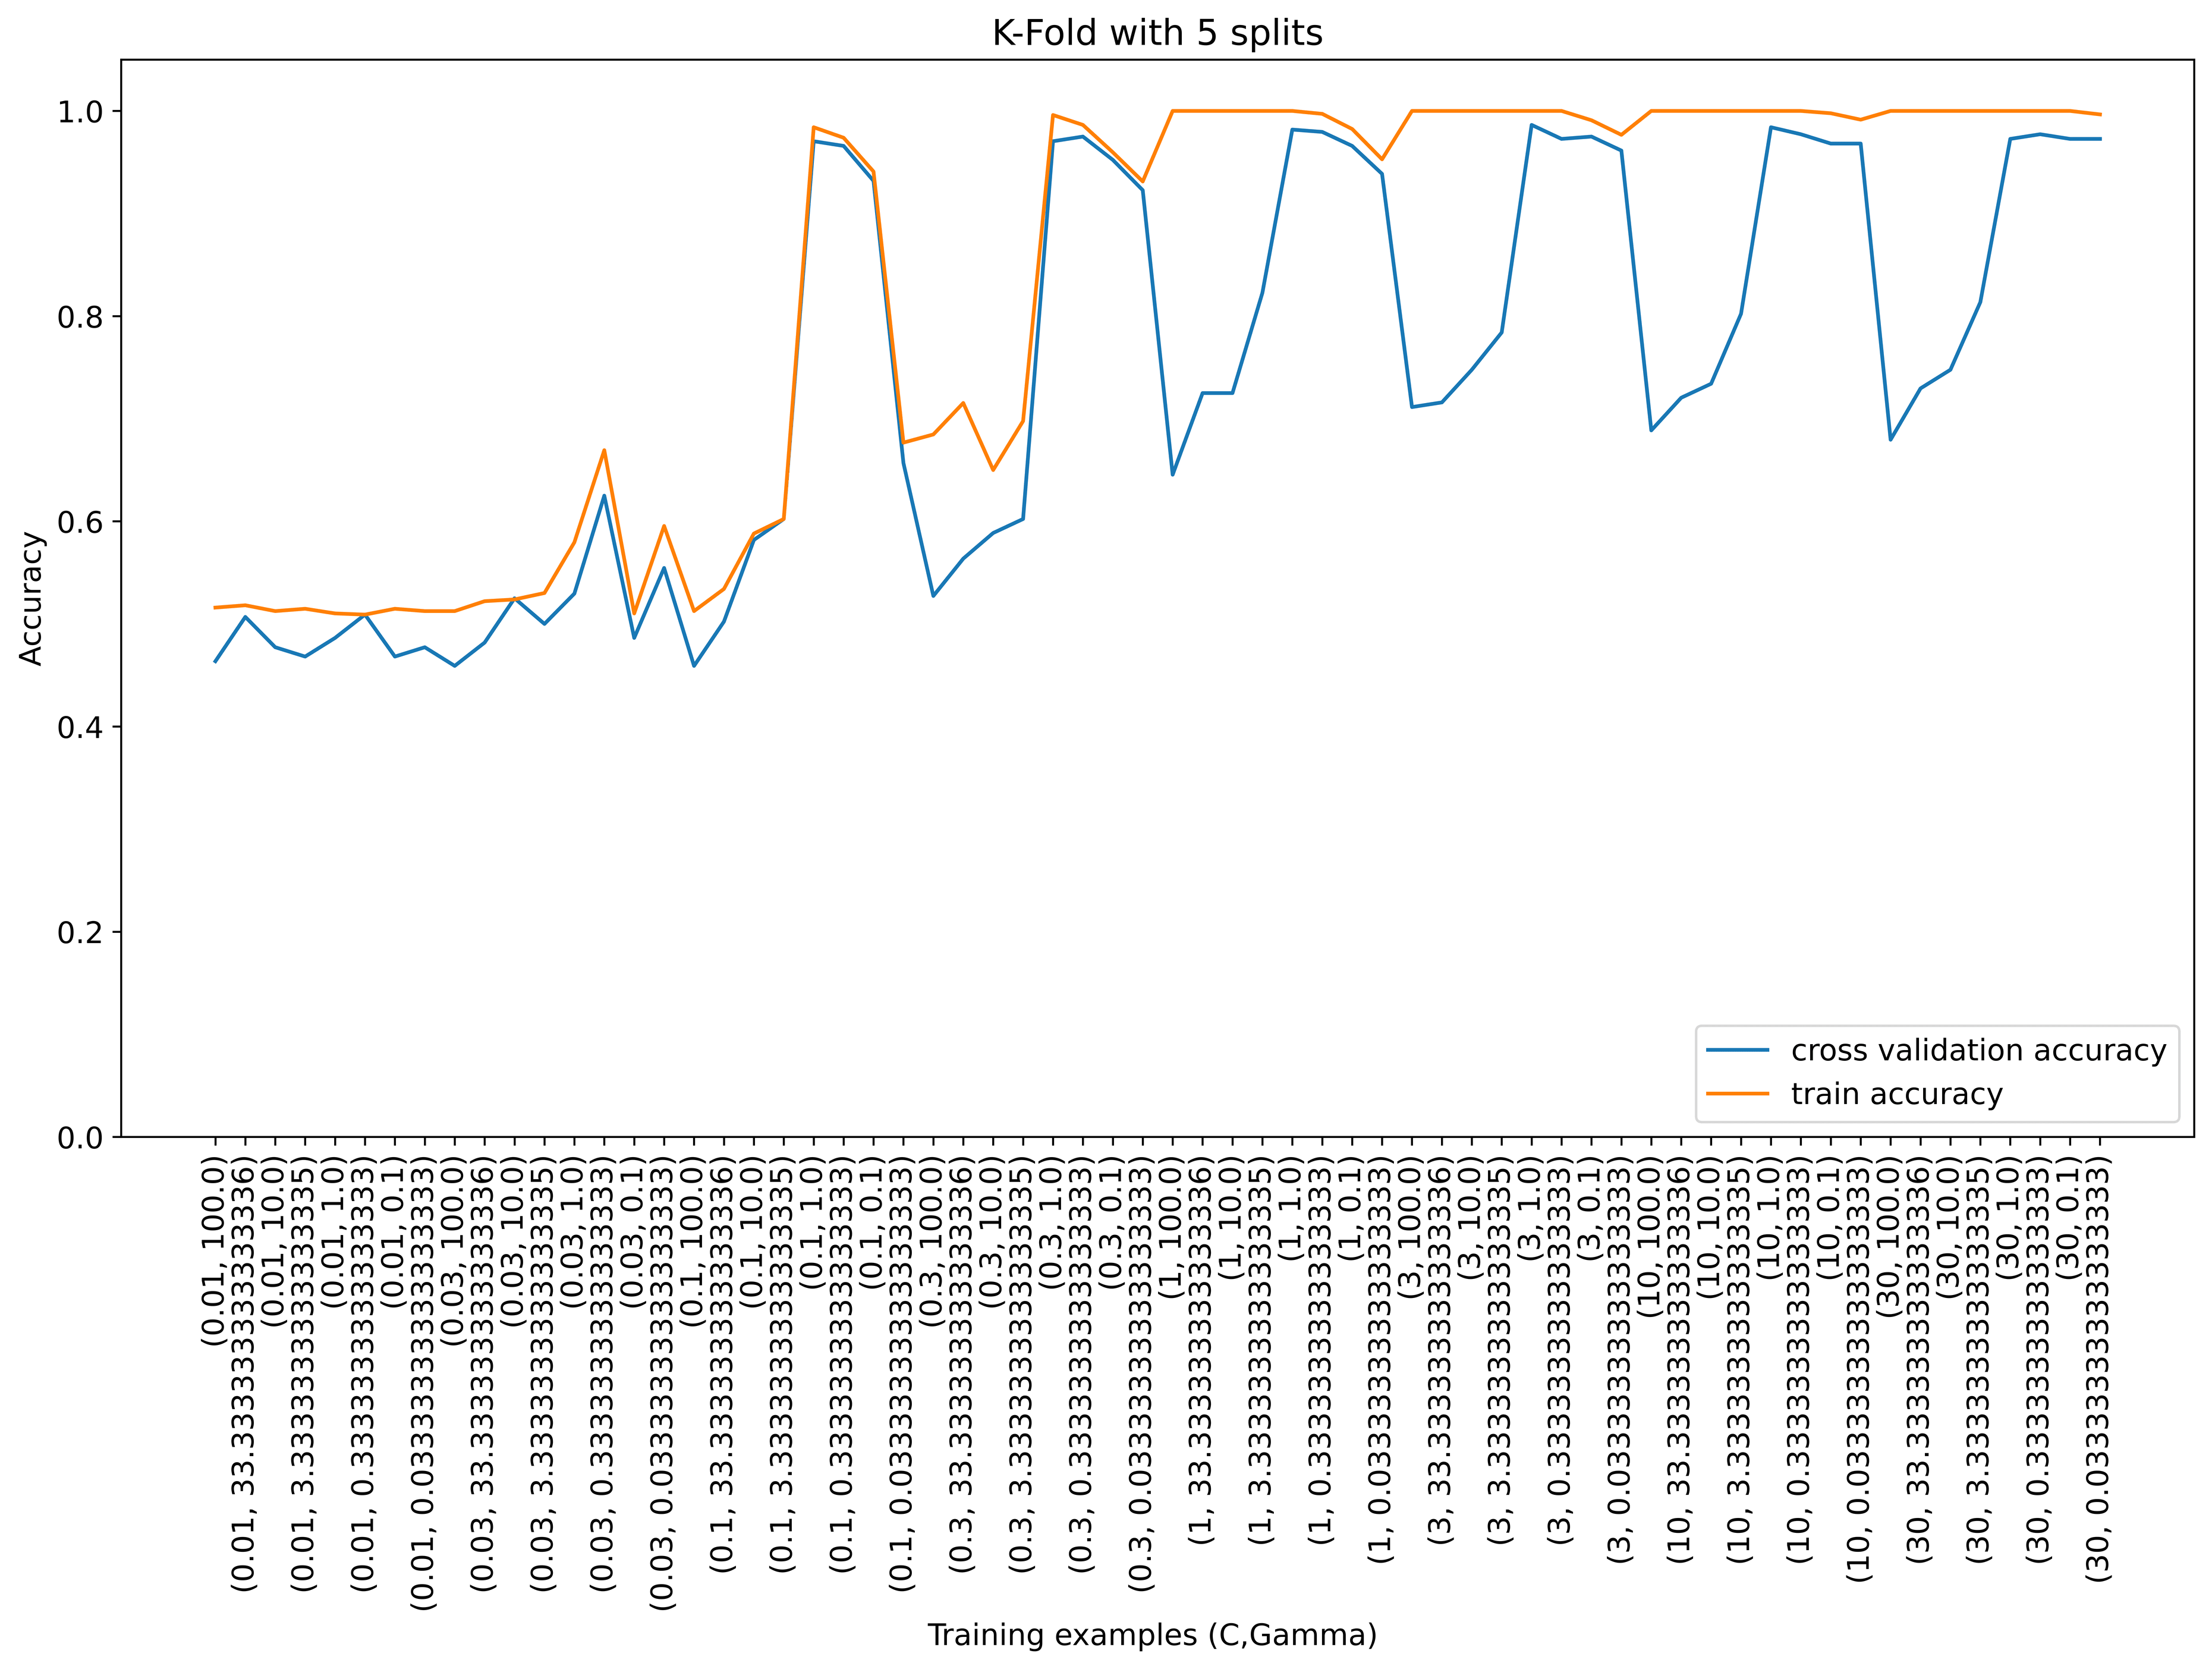
\includegraphics[width=1\linewidth]{images/svm_cross_validation.png}}
\caption{SVM - Cross-Validation using multiple values for C and Gamma}
\label{fig:svm-cross-validation}
\end{figure}

Based on the Cross Validation data, we created an SVM model with a Radial Basis Function (RBF) kernel, and with the hyper-parameters C = 30 and Gamma = 1, that returns 1 when the image is a face, and 0 otherwise, as we can see in table \ref{table:svm-final-configuration}.

\begin{table}[htbp]
\centering
\caption{SVM - Final Configuration}
\begin{tabular}{ |c|c| } 
 \hline
 \textbf{Train Data} & 80\% \\ 
 \hline
 \textbf{Test Data} & 20\% \\ 
 \hline
 \textbf{Kernel} &  Radial Basis Function (RBF) \\ 
 \hline
 \textbf{Gamma} & 1 \\ 
 \hline
 \textbf{C} & 30 \\ 
 \hline
\end{tabular}
\label{table:svm-final-configuration}
\end{table}

Finally, to ensure that the model didn't end up in a local minimum, and that our model was actually learning we run the all process 50 times and calculated the mean values to both train and test phases.
